\documentclass[11pt,en]{elegantpaper}
\usepackage{gensymb}
\usepackage{float}


\title{GAN based semi-supervised learning crop disease classifier}
\author{Wangzhihui Mei 2019124044 Chang Xu 2019180034 \\ Zijia He 2019124057 Hongyi Huang 2019180029}
\institute{CCNU-UOW JI}

\version{}
\date{}


\begin{document}

\maketitle

\begin{abstract}
	this paper uses semi-supervised generative adversarial networks to perform semi-supervised learning on crop disease and insect images. We redesigned the network composition of generators and discriminators in generative adversarial networks based on the characteristics of crop images. In the generative confrontation network used, this paper designs a multi-layer generator network and a discriminator deep neural network.
\end{abstract}

\section{Introduction}

As a big agricultural country, China suffer biological disasters such as disease and insect Tons annually. The crop diseases, insects, and grass diseases are not only diverse and widely distributed, but also have complicated disaster conditions\cite{hsu2019food}. This directly affects the sustainable and stable development of agriculture and the growth of the rural economy. Practice has shown that the rational application of pesticides is an important measure to ensure a bumper harvest in agriculture, and the premise of rational application of pesticides is the correct diagnosis of the types and occurrence of pests and diseases. Not only is it impossible to obtain a good agricultural harvest, it will also cause a series of more serious problems. At present, the identification of pests and diseases still mainly rely on manual or semi-manual identification, which is actually a highly repetitive and time-consuming task. As an important subfield in artificial intelligence, machine learning plays a key role in modern intelligent technology. We can also use machine learning technology to detect crop diseases and insect pests, thereby saving manpower and achieving information agriculture\cite{mahlein2016plant}.

For machine learning, according to the specific conditions of labeled and unlabeled samples contained in the training set, the task types can be roughly divided into the following types: supervised learning, unsupervised learning, and semi-supervised learning. In supervised learning, the classifier learns a large number of labeled training samples to build a model for predicting the label of unseen samples. "Label" refers to the output corresponding to the sample. In the classification problem, the label is the category to which the sample belongs, and in regression analysis, the label is the real-value output corresponding to the sample. With the rapid development of data collection and storage technology, it has been quite easy to collect a large number of unlabeled samples, and obtaining a large number of labeled samples is relatively difficult, because obtaining these labels may require a lot of manpower and material resources. There are also a large number of such cases in detection of crop diseases and insect pests. Relevant agencies have a large number of unlabeled data, and only a small number of representative samples can be labeled by human labor, but all labeling is not realistic. In fact, there are a lot of such situations in crop disease and pest monitoring. The relevant agricultural management agencies have a large amount of unlabeled data, but if all these images are required to be labeled, the workload is extremely large and often unrealistic.

Semi-supervised learning (SSL)\cite{rasmus2015semisupervised}came into being under the above background and has become an important research field in pattern recognition and machine learning. In recent years, with the extensive application of machine learning theory in data analysis and data mining, such as web page and text classification, image and video retrieval, medical data processing, etc., semi-supervised learning has made great progress in theoretical research and practical applications . The research of semi-supervised learning mainly focuses on how to obtain a learner with good performance and generalization ability when part of the training data is missing. The lack of information here includes the absence of category labels or the presence of noise, and the lack of some feature dimensions of the data. The theoretical research of semi-supervised learning provides us with an in-depth understanding of many important theoretical issues of machine learning, such as the relationship between data manifolds and data categories, the proper handling of missing data, the effective use of labeled data, and the relationship between supervised and unsupervised learning Connection, the design of active learning algorithms, etc. have very important guiding significance.

% With the recent rapid development of data availability, computing power and new algorithms, machine learning has gradually become one of the key methods for implementing artificial intelligence (AI). 
% Machine learning is a subset of artificial intelligence in the broader field of computer science. It uses computers and algorithms to learn from "data" and 
% discover "patterns and insights," because in many cases, "patterns and insights" are hidden in "data." Traditional machine learning is divided into two categories: supervised learning and unsupervised learning. Supervised learning refers to training 
% models on known input and output data so that they can predict future output data, while unsupervised learning finds hidden patterns or inherent structures in input data, Which means that the characteristic of unsupervised learning is that the training samples are unlabeled, 
% and supervised learning is directed to the labeled training set. Semi-supervised learning is a learning method that combines supervised learning with unsupervised learning. Given a set of labeled samples: $\mathbb{D}_{l}=\left\{\left(\overrightarrow{\mathbf{x}}_{1}, y_{1}\right),\left(\overrightarrow{\mathbf{x}}_{2}, y_{2}\right), \cdots,\left(\overrightarrow{\mathbf{x}}_{l}, y_{l}\right)\right\}$
% And unlabeled sample collection:$\mathbb{D}_{u}=\left\{\left(\overrightarrow{\mathbf{x}}_{l+1}, y_{l+1}\right),\left(\overrightarrow{\mathbf{x}}_{l+2}, y_{l+2}\right), \cdots,\left(\overrightarrow{\mathbf{x}}_{l+u}, y_{l+u}\right)\right\}$, The learner automatically uses unlabeled $\mathbb{D}_{u}$ to improve learning performance\par
% According to the angle of statistic theory, Inductive SSL includes two types of models: Transductive SSL and Inductive SSL. Transductive SSL to process only the given training data in the sample space, use the samples with class labels and the examples without class labels in the training
% data to train, predict the class labels of the examples without class labels in the training data; SSL processes all the given and unknown samples in the entire sample space, and simultaneously uses the samples with class labels and the samples without class labels in the training data, and the unknown test samples to train together, not only predicts the classlessness in the training data 
% the class label of the sample of the label, the more important is to predict the class label of the unknown test sample\cite{sun2013rgb}. SSL has been used to solve many practical problems, Yarrowsky uses collaborative training to construct different classifiers from the two views to disambiguate the meaning of the word. One classifier uses the context of the word in the text, and the other classifier is based on the meaning of the word that appears elsewhere in the text;
% Zhou and others used collaborative training for image retrieval; Goldberg and Zhu\cite{zhu2002learning} used a graph-based method to solve the problem of emotional grading;

\section{Background theory}
The research history of SSL can be traced back to the 1970s. During this period, Self-Training, Transdictionary Learning, Generative Mode and other learning methods appeared. 
The study of SSL became more fanatical in the 1990s, the emergence of new theories, and the development of new applications in natural language processing, text classification, and computer vision have promoted the development of SSL and emerged collaborative training New methods and Transient SupportSupperPortVechorMachine(TSVM) and other new methods.
Merz et al. Proposed the term SSL in 1992 and used SSL for classification problems for the first time. Today, semi-supervised learning algorithms are mainly divided into 4 categories, which still has huge potential in the field of machine learning.
\subsection{Generative Methods}
Generative semi-supervised learning method is a method based directly on generative model. Generative semi-supervised learning(GSSL) assumes that all data (whether or not labeled) are generated by the same underlying model.
\begin{itemize}
	\item This assumption makes it possible to associate unlabeled samples with learning objectives through the parameters of the latent model.
	\item The labeling of unlabeled samples can be regarded as the missing parameter of the model, which can usually be solved based on the maximum likelihood estimation based on the EM algorithm.
\end{itemize}
Models\cite{li2020mixture} for generating examples include Gaussian models, Bayesian networks, Sigmoid BeliefNetWorks, GMM, Multimedia Mixture Model(MMM), and Hidden Markov Model(HMM).
\begin{enumerate}
	\item The examples in the Gaussian model follow the Gaussian distribution: \\
		$p(\boldsymbol{x} | y)=N(\boldsymbol{x} | \boldsymbol{\mu}, \boldsymbol{\Sigma})=\frac{1}{(2 \pi)^{D / 2}|\boldsymbol{\Sigma}|^{1 / 2}} \exp \left(-\frac{1}{2}(\boldsymbol{x}-\boldsymbol{\mu})^{\mathrm{T}} \boldsymbol{\Sigma}^{-1}(\boldsymbol{x}-\boldsymbol{\mu})\right)$
	\item The probability distribution of the samples in the Bayesian network is shown in the figure: \\
		\begin{figure}[H]
		\centering
		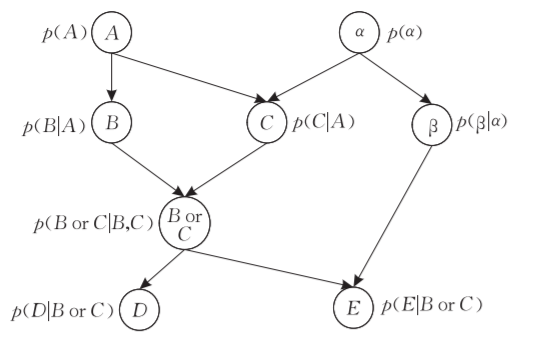
\includegraphics[scale=0.4]{figure/bys.png}
		\caption{Bayesian Network}
		\end{figure}
	\item The samples in the S-type belief network obey the probability distribution:\\
	$p\left(\boldsymbol{x}_{i} | p a\left(\boldsymbol{x}_{i}\right)\right)=\frac{\exp \left(\left(\sum_{j} \boldsymbol{J}_{i j} \boldsymbol{x}_{j}+h_{i}\right) \boldsymbol{x}_{i}\right)}{1+\exp \left(\sum_{j} \boldsymbol{J}_{i j} \boldsymbol{x}_{j}+h_{i}\right)}$
	\item GMM is a mixed distribution model of multiple Gaussian distributions, assuming that the sample is generated by weighted mixing of multiple models $\sum_{i} \pi_{i} p_{i}(\boldsymbol{x} | y)$, $\sum_{i} \pi_{i}=1$.Each model follows a Gaussian distribution.
	\item MMM is a mixed distribution model of multiple multi-modal distributions, assuming that the sample is generated by the weighted mixture of multiple models, The distribution of each model follows the multimodal distribution $p\left(\boldsymbol{x}=\left(x_{\cdot 1}, \cdots, x_{\cdot d}\right) | \boldsymbol{\mu}\right)=\frac{\left(\sum_{i=1}^{D} x_{\cdot i}\right) !}{x_{\cdot 1} ! \cdots x_{\cdot D} !} \prod_{d=1}^{D} \mu_{d}^{x_{\cdot d}}$
	\item HMM is used to build a model of the sample sequence. The transition probability matrix between the specified states is transferred from one state to another state at a certain period to form the sequence. Each sample in the sequence is generated by the hidden state, where the state condition distribution can be Gaussian Mixed distribution or multi-modal mixed distribution. The current state depends only on the previous state, and the output only depends on the current state.
\end{enumerate}

The advantages of generative semi-supervised learning method: the method is simple and easy to implement. In the case of very little labeled data, it often performs better than other methods.
Disadvantages: The model assumption must be accurate, that is, the assumed generative model must be consistent with the real data distribution, otherwise the use of unlabeled data will reduce the generalization performance.

\subsection{Discriminative Methods}
The discriminative method\cite{zhang2017label} uses the maximum interval algorithm to simultaneously train class targetsThe signed sample and the sample without class label learning decision boundary, as shown belowAs shown, make it pass through the low-density data area, and make the learnedThe distance between the classification hyperplane and the nearest sample is the largest.
\begin{figure}[H]
		\centering
		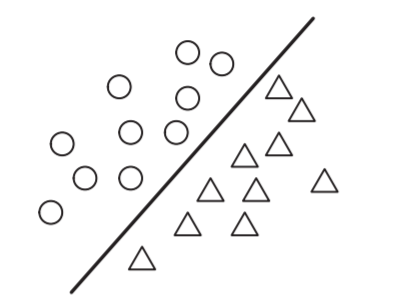
\includegraphics[scale=0.4]{figure/2.png}
		\caption{Schematic diagram of discriminant method}
\end{figure}
Discriminant methods include LDA\cite{alshehhi2017hierarchical}, generalized discriminant analysis (GenerarizedDiscriminantAnalysis (GDA), semi-supervised supportVector machine (Semi-SuppliedSupperPortVecutorMachine,SVM), entropy regularization method and KNN method.
\begin{enumerate}
\item LDA is also called Fisher Linear Discrimination (Fisher Liner)
Discriminative Analysis (FDA), originally developed by Fisher
It was proposed in 1936 that the basic idea is to project the sample to the appropriate dimension
In the low-dimensional space of, the projected sample has in the new subspace
The largest inter-class distance and the smallest intra-class distance, that is, the sample according to the class
Don't be divided into many clusters.
\item Badat and Anouar send LDA
Expand to multiple types of problems, put forward GDA. Through a nonlinear mapping, the
sample is mapped to a high-dimensional feature space and used in this feature space
FDA training. When LDA and GDA are used for SSL, there is a
the value of the class label of the divided sample is unknown, and the goal is to request the solution of the class value of the label.Because of $y_{i} \in\left\{c_{1}, c_{2}, \cdots, c_{C}\right\}$,this is a Mixed integer programming problem.
\item TSVM was originally proposed by Vapnik and Sterin for Linear prediction function for estimating class labels $f(x)=w^{\top} x+b$.Since it can also be used to estimate the class labels of unknown test samples, what is actually obtained is the decision boundary on the entire sample space. It is not a strict direct push method, but an inductive semi-supervised method, so it is called SVMs.TSVM attempts to consider various possible label assignments for unlabeled samples:
\begin{itemize}
	\item Trying to use each unlabeled sample as a positive or negative example.
	\item Then, in all these results, we seek a partitioned hyperplane that maximizes the spacing between all samples (including labeled samples and unlabeled samples with label assignment).
	\item Once the dividing hyperplane is determined, the final label assignment for unlabeled samples is its prediction result.
\end{itemize}
Sample set of given markers $\mathbb{D}_{l}=\left\{\left(\overrightarrow{\mathbf{x}}_{1}, y_{1}\right),\left(\overrightarrow{\mathbf{x}}_{2}, y_{2}\right), \cdots,\left(\overrightarrow{\mathbf{x}}_{l}, y_{l}\right)\right\}$ and Unlabeled sample set $\mathbb{D}_{u}=\left\{\overrightarrow{\mathbf{x}}_{l+1}, \overrightarrow{\mathbf{x}}_{l+2}, \cdots, \overrightarrow{\mathbf{x}}_{l+u}\right\}$ among them $l \ll u, l+u=N, y_{i} \in\{-1,+1\}, i=1,2, \cdots, l$.The goal of TSVM learning is to give prediction labels for the samples in $\mathbb{D}_{\boldsymbol{u}}$.\\
$\hat{\overrightarrow{\mathbf{y}}}=\left(\hat{y}_{l+1}, \hat{y}_{l+2}, \cdots, \hat{y}_{l+u}\right)^{T}, \hat{y}_{i} \in\{-1,+1\}, i=l+1, l+2, \cdots, N$ makes:
\begin{equation}\begin{array}{c}
\min _{\overrightarrow{\mathbf{w}}, b, \hat{\mathbf{y}}, \vec{\xi}} \frac{1}{2}\|\overrightarrow{\mathbf{w}}\|_{2}^{2}+C_{l} \sum_{i=1}^{l} \xi_{i}+C_{u} \sum_{i=l+1}^{N} \xi_{i} \\
s . t . y_{i}\left(\overrightarrow{\mathbf{w}}^{T} \overrightarrow{\mathbf{x}}_{i}+b\right) \geq 1-\xi_{i}, \quad i=1,2, \cdots, l \\
\hat{y}_{i}\left(\overrightarrow{\mathbf{w}}^{T} \overrightarrow{\mathbf{x}}_{i}+b\right) \geq 1-\xi_{i}, \quad i=l+1, l+2, \cdots, N \\
\xi_{i} \geq 0, \quad i=1,2, \cdots, N
\end{array}\end{equation}
Among them:
\begin{itemize}
	\item $(\vec{w}, b)$ defines a dividing hyperplane.
	\item $\vec{\xi}$ is the relaxation vector:
	\begin{itemize}
		\item $\xi_{i}, i=1,2, \cdots, l$ corresponds to the marked sample.
		\item $\xi_{i}, i=l+1, l+2, \cdots, N$ corresponds to the unlabeled sample.
	\end{itemize}
	\item $C_{l},C_{u}$ are the compromise parameters specified by the user to balance the complexity of the model, the importance of marked samples, and the importance of unlabeled samples.
\end{itemize}
\item Entropy regularization method uses Shannon conditional entropy to measure the degree of overlap between classes, and its objective function is:
\begin{equation}\begin{array}{l}
\max _{\theta} \frac{1}{2}\|w\|^{2}+C_{1} \sum_{i=1}^{l} \ln p\left(y_{i} | \boldsymbol{x}_{i}, \theta\right)+
\lambda \sum_{i=l+1}^{n} \sum_{y_{i}=\tau_{1}}^{c_{c}} p\left(y_{i} | \boldsymbol{x}_{i}, \theta\right) \ln p\left(y_{i} | \boldsymbol{x}_{i}, \theta\right)
\end{array}\end{equation}
\item The KNN method finds the k nearest neighbor samples that are closest to the test sample in all samples, and the number of each type are $k_{j}$,$j=c_{1}, \cdots, c_{C}$,using decision rule $\arg \max _{j} k_{j}, j=c_{1}, \cdots, c_{C}$ to select the class label to mark the sample.
\end{enumerate}
\subsection{Graph-Based Methods}
The essence of the graph-based method\cite{chen2018survey} is label propagation (LabelPropagation). Based on the manifold hypothesis, the graph is constructed according to the geometric structure between the samples. The graph nodes are used to represent the samples. Propagate the class label from the sample with class label to the sample without class label.


The basic training process of the graph-based method\cite{chong2020graph} is:
\begin{itemize}
	\item Choosing an appropriate distance function to calculate the distance between samples. The available distance functions include Euclidean distance, Manhattan distance, Chebyshev distance, Ming's distance, Mahalanobis distance, and normalized Euclidean distance;
	\item According to the calculated distance, select an appropriate connection method, connect the samples with edges, and construct a connection diagram. The constructed connection graph is divided into dense graph (DenseGraph) and sparse graph (SparseGraph). The typical representative of dense graph is a fully connected graph, as shown in Figure 3, there are edge connections between any two nodes; sparse as shown in Figure 4, according to a certain criterion, the closest nodes are connected, including KNN diagram, $\varepsilon$-Nearest Neighbor ($\varepsilon$NN) diagram, tangent weight diagram, exponential weight diagram, etc ;
	\begin{figure}[H]
		\centering
		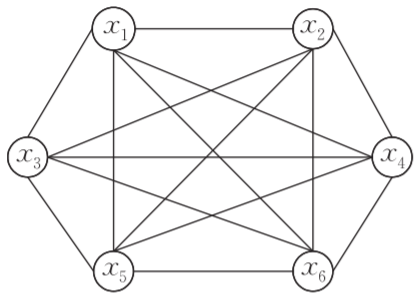
\includegraphics[scale=0.4]{figure/3.png}
		\caption{Full connection diagram}
	\end{figure}
	\begin{figure}[H]
		\centering
		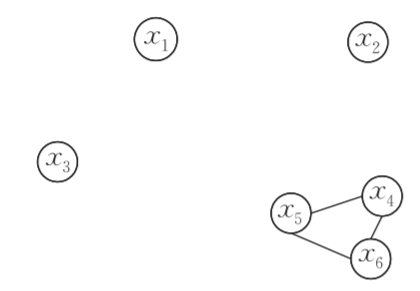
\includegraphics[scale=0.4]{figure/4.png}
		\caption{Sparse graph}
	\end{figure}
	\item Kernel function is used to assign weights to the connected edges of the graph. The weights reflect the similarity between the two nodes connected by this edge. When the two nodes are $ \ boldsymbol {x} _ {i } $ And $ \ boldsymbol {x} _ {j} $ are very close, the weight $ w_ {ij} $ of the edge connecting these two nodes is very large, these two examples have the same class label The probability is very large; conversely, when the two nodes are $ \ boldsymbol {x} _ {i} $ and $ \ boldsymbol {x} _ {j} $ are very far away, the edge connecting the two nodes The weight $ w_ {ij} $ is very small, and the probability of these two samples having the same type of label is very small. Commonly used kernel functions include linear kernel, polynomial kernel, Gaussian kernel, radial basis kernel, hyperbolic tangent kernel, neural network kernel, Fisher kernel and spline kernel;
	\item Determine and solve the optimization problem according to the learning objective. The goal of the semi-supervised classification problem is to find the prediction function $ f (x) $ of the class label that minimizes the objective function. This problem can be seen as a regularization risk minimization of a composite objective function consisting of a loss function and a regularization function Problem, the objective function for solving semi-supervised classification problems based on graph-based methods is generally expressed as:
	\begin{equation}\min _{f(x)} V(y, f(x))+\lambda \Omega(f)\end{equation}
	In equation (3), the loss function $ V (y, f (x)) $ is used to penalize the case where the predicted class label of the sample is not equal to the given class label. The smoothness of the function makes the predicted class labels of the nearest neighbors the same. According to the specific learning task, different loss functions and regularization functions can be selected. For example, the loss function can be the square error function, absolute value function, logarithmic function, exponential function, and hinge loss function. Generally, the loss function and the regularization function are limited to the re-copy kernel Hilbert space (Reproducing Kernel Hierarchy Spare, RHKHS), and the learning machine is solved with a nuclear learning algorithm.
\end{itemize}
The following are some typical Graph-Based Methods:
\begin{enumerate}
	\item In 2001, Blum and Chawla proposed the first graph-based SSL method-the minimum cut method (Mincut), which regards the samples marked as positive as the source node and the samples marked as negative as the target node Point, find a group of edges, so that after removing these edges, there is no connection between the source node and the target node, that is, the graph is divided into two independent clouds, and this group of edges is called a graph cut (Cut). After the graph is segmented, the label of the node class connected to the source node is marked as positive, and the label of the node class connected to the target node is marked as negative. This method selects the square loss with infinite weight as the loss function $V(y, f(\boldsymbol{x}))=\infty \cdot \sum_{i=1}^{l}\left(y_{i}-f\left(\boldsymbol{x}_{i}\right)\right)^{2}$,represent regularization function with cut size $\Omega(f)=\boldsymbol{f}^{\mathrm{T}} L \boldsymbol{f}$ and limited to any node with class label $ x_ {i} $, the predicted class label is equal to the given class label $f\left(\boldsymbol{x}_{i}\right)=y_{i}$
	\item In 2003, Zhu et al. Proposed the harmonic function method (Harmonic Function), also known as the Gaussian random field method (Gauss Random Field), to establish the distribution model of the prediction function on the graph, thereby expanding the discrete prediction function into a continuous prediction function. Like the minimum cut method, this method also chooses the square loss with infinite weight as the loss function. The size of the cut represents the regularization function. The difference is that the prediction function takes continuous values, rather than directly equals the class label value. The classification probability of the example solves the problem that the minimum cut method cannot solve.
	\item Yan and Wang proposed a new SSL structure based on the $ l_ {1} $ graph. The idea of the $ l_ {1} $ graph comes from the fact that each data can be reconstructed by sparse linear superposition of training data, by The $ l_ {1} $ optimization problem obtains the sparse reconstruction coefficients, and uses the obtained coefficients to infer the weight of the directed $ l_ {1} $ graph, and simultaneously obtains the $ l_ {1} $ graph in a parameter-free manner. Near-neighbor structure and weights, and face recognition and image classification experiments, the implementation results show that the performance of this method is superior to the traditional graph method.
\end{enumerate}

\section{Application}

There are two commonly used hypotheses in the field of semi-supervised learning: the cluster hypothesis and the manifold hypothesis. The clustering hypothesis refers to that the samples in the same cluster have a larger possibility of having the same mark, which means that the interface of different mark points should not appear in the area with a higher sample density while the manifold hypothesis means that adjacent samples have similar properties, and their labels should also be similar\cite{shen2003multilabel}. Since both the graph method and the density-based clustering method adhere to these two assumptions, the combined effect of the two methods on a certain level should be comparable to the graph method alone. Specifically, the computational complexity of the graph method is higher, but the computational complexity of the local density estimation is much lower. Our picture uses the advantage of local giant thunder in computing time to reduce the composition of the node tree, on the other hand The method has a good classification effect on the overall characterization ability of the data structure.



According to this, we are completing unsupervised learning by labeling a small number of images and performing label propagation.

\subsection{Preprocessing}
Image preprocessing is an important link in the process of disease recognition. It is a kind of pre-processing relative to feature extraction and image recognition. As the actual production process, the collection equipment and environmental parameters are very different, there will be problems such as noise interference, low contrast, unclear targets, and interference from unrelated objects\cite{rechcigl2018environmentally}. 

Pre-processing means that the chicken takes out the appropriate transformation of the image according to the actual situation to highlight some useful information and remove disturbing information. Therefore, we need to perform some tricky transformation to initial crop images.

\subsubsection{Grayscale Conversion}
Images are commonly saved by RGB(i.e. Red, Green and Blue) channels, which can preserve the natural color while reducing the memory consumption of the storage. Some researcher has done some related work\cite{sun2013rgb}, by extracting G-channel elements, they can not only simplify the algorithm, but also retain the original information of the image on the original basis. In this article, we also applied weighted sum conversion based on asymmetric weights. We increased the weight of G channel and reduce the weight of RB channels. 
$$Gray_{img}=R\times 0.287+G\times 0.599 + B\times 0.114$$
R,G,B represent Red,Green and Blue channel. The conversed image kept a lot of original information from initial image.

\subsubsection{Image standardization and normalization}
In the original crop image, the floating range of pixel values ​​is large, which results in the objective function of the classification algorithm being unable to handle the features of the original image well in a large range. That is to say, assuming that a certain feature value in the original image has a large value range, such feature value will affect the final classification accuracy. Therefore, before classification, it is necessary to make a relatively standardized adjustment to his images, limiting the feature values ​​to a certain range, to maintain a relative balance between the original characteristics. In this article, we applied image normalization. $X_mid$ is a middle variable to simplify the formula, $X$ is pixel matrix, $N$ is the total pixel num in the image, $X_i$ is the value of pixel with the index $i$.
$$X_{mid}=\frac{X-\frac{1}{N} \sum_{i=1}^{N} x_{i}}{\sqrt{\frac{1}{N} \sum_{i=1}^{N}\left(x_{i}-\frac{1}{N} \sum_{i=1}^{N} x_{i}\right)^{2}}}$$ 
$$X_{norm}=\frac{X_{mid}-\min \left(X_{mid}\right)}{\max \left(X_{mid}\right)-\min \left(X_{mid}\right)} \times 255$$

\subsection{Feature extraction}
Crop diseases and insect pests will change the characteristics of the original plant tissue, including texture features and color features. The texture feature is a visual feature that does not depend on the color or brightness of the homogenous phenomenon in the image. It contains important information on the surface structure of the object and their relationship with the surrounding environment. Researchers can find other images with similar textures by submitting images containing certain textures. Color is the most prominent feature of people's sensory color images. Compared with other features, color features are relatively stable, are insensitive to image rotation, translation, and scale changes, and have good adaptability\cite{mohanty2016using}.
$$D_{B}=\frac{D_{max} }{A_{0}} \sum_{i=0}^{D_{A}} H_{i} \quad\left(D_{A}=0,1,2, \ldots, L-1\right)$$

The conversion is simple, fast and effective, and has been widely used.
\subsubsection{Color feature}
Color is an important feature descriptor of image processing. When plants are attacked by diseases and insect pests, the abnormal areas of their images often change color. Construct. Based on this, we can construct histograms in different color spaces for feature extraction. After histogram equalization, the image may be insensitive to local differences in brightness, reducing the impact on classification results due to differences in image brightness. The pixels in the image after equalization occupy as many gray levels as possible and are evenly distributed,so that the processed image will have a large contrast and dynamic range\cite{guo2017color}. The formula of histogram equalization algorithm is as follows($D_B$ is the transformed gray value, $D_max$ is the maximum gray value in the picture, $A_0$ is the total number of the pixels, $D_A$ is the gray value before transformation, $H_i$ is the number of pixels with ith gray value, $L$ is the maximum pixel level in the image). 
\begin{figure}[h]
	\centering
	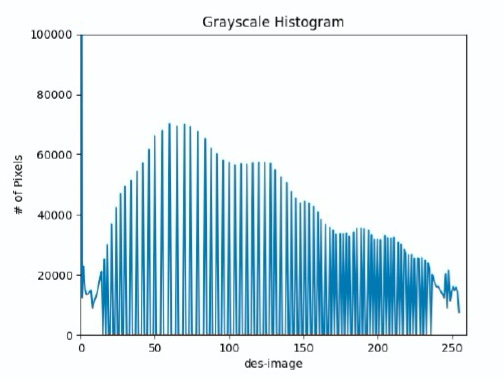
\includegraphics[width=0.7\textwidth]{figure/grayscalehistogram}
	\caption{The grayscale histogram}
\end{figure}

\subsubsection{Texture feature}
Texture is a visual feature that reflects the homogeneous phenomenon in the image, and texture analysis is the extraction and analysis of the gray scale spatial distribution pattern of the image. Texture features are different from image features such as gray scale and color\cite{humeau2019texture}. It is expressed by the gray scale distribution of pixels and their surrounding spatial neighborhood. The texture feature embodies the property of the surface structure and arrangement of the surface structure that changes slowly or periodicatwo.

we extract the following two texture features from each crop image:
\begin{enumerate}
	\item Gray level co-occurrence matrix: statistical texture features based on gray level co-occurrence matrix (GLCM). This feature is based on the gray attributes of pixels and their neighborhoods, and the statistical features in the texture area are studied. The gray level co-occurrence matrix is defined by the joint probability density of the pixels at two positions, and can reflect the comprehensive information of the image gray level about the direction, adjacent interval, and change range. In this paper, the gray level co-occurrence matrix of $\theta = 0^{\circ},45^{\circ},90^{\circ},135^{\circ}$ is first extracted, and then the energy, contrast, correlation, entropy and inverse gap are five typical parameters that can intuitively reflect the texture condition described by the co-occurrence matrix, and 20 feature values are extracted from an image.
	\begin{gather}%会产生编号
		ASM=\sum_{i} \sum_{j} P(i, j)^{2}\\
		CON=\sum_{i} \sum_{j}(i-j)^{2} P(i,j)\\
		COR=\sum_{i} \sum_{j} \frac{\left(i-\mu_{i}\right)\left(j-\mu_{j}\right)}{\sigma_{i} \sigma_{j}} P(i, j)\\
		ENT=-\sum_{i} \sum_{j} P(i, j) \log P(i, j)\\
		IDM=\sum_{i} \sum_{j} \frac{P(i, j)}{1+(i-j)^{2}}
	\end{gather}
	\item Gray gradient co-occurrence matrix: The gray gradient co-occurrence matrix model mainly reflects the relationship between the two most basic elements in the image, namely the gray level and the gradient (or edge) of the image point. The gray level of each image point is the basis for forming the image, and the gradient is the element that forms the edge contour of the image. The main information of the image is provided by the edge contour of the image. The gray gradient space clearly describes the resolution law of the gray and gradient of each pixel in the image, and also gives the spatial relationship between each image point and its field image point. It can describe the image texture well and reflect the direction texture from the gradient direction. The classification result of the gray-level gradient co-occurrence matrix is superior to the gray-level co-occurrence matrix, because the gray-level co-occurrence matrix uses only gray-scale information, while the gray-scale gradient co-occurrence matrix uses both the gray-scale and gradient information of the image. Gray gradient co-occurrence matrix (GGCM) texture feature analysis is to extract the texture features of gray gradient co-occurrence matrix. The gradient information of the image is added to the gray level co-occurrence matrix, so that the co-occurrence matrix can better contain the elements of the texture image and their arrangement information.
\end{enumerate}

\subsection{GAN based classifier}
The network structure of the generative adversarial network includes a generative model G and a discriminant model D\cite{ledig2017photo}. The role of the generated model is to be able to capture the distribution of data from the training sample data, and the discriminant model implements the function of a $(n + 1)$ classifier classification model ($n$ represents the original number of categories in the training data, and $n +1$ categories are added true and false categories), to determine whether the data input to the discrimination model is real data or sample data generated by the generation model. The optimization process of generating an adversarial network can be understood as a "minimax two-player game" problem. During training, one of the generated model and the discriminant model is fixed, and the parameters of the other model are updated. Iterate alternately, and update the parameters to maximize the error of the other model. Eventually, generator G can estimate the distribution of sample data, and can generate samples that are very similar to the distribution of training data, and discriminator D will be a great Discriminator\cite{zhao2016energy}.

\subsubsection{How GAN perform Semi-supervised learning}
In this topic, this paper uses Generative Adversarial Network (GAN) to implement a semi-supervised learning algorithm based on deep learning. Unlabeled sample data does not have any category information, so it is not possible to conduct supervised model training, but the role of the generator in generating an adversarial network is to generate pseudo samples from random signals for the true and false classification performance of the discriminator Training, so in the semi-supervised generation adversarial network, compared to the pseudo samples generated by the generator in the network, the unlabeled sample data has a label, that is, the real sample, because this part of the sample is taken from the real The crops suffering from pests and diseases are not generated by the generator, so that the discriminator D can be trained together with the pseudo samples. The distribution of such network training data is shown in Figure \ref{datadist}.
\begin{figure}[H]
    \centering
	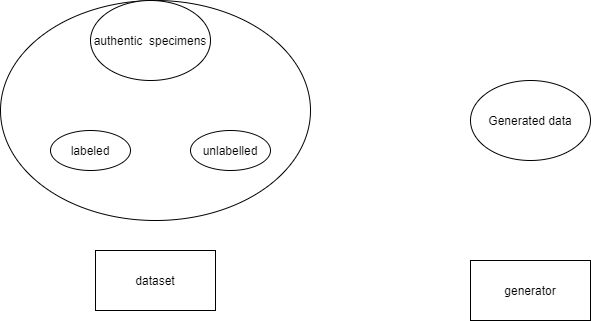
\includegraphics[scale=0.5]{figure/5.1.png} 
	\caption{Dataset distribution}
	\label{datadist}
\end{figure}
As shown in the Figure \ref{datadist}, the data with samples and the data without samples form the real data class, and the pseudo samples generated by the generator form the generated data class, that is, the data set that belongs to the false label.

Therefore, the data in the training set contains two parts, one is the original labeled data $x$, and the other is the unlabeled real crop (after image feature extraction) data $x_u$, the generator will generate $I_f$ pseudo from random noise sample. When the discriminator in the network inputs the sample $I$, for the 2-classification problem of this topic, the discriminator will output $2+1$ dimensional estimate $L$, and finally pass the $softmax$ function. The probability $P$ of the category, the first 2 dimensions correspond to the original 2-category category, and the last dimension corresponds to whether the sample is a pseudo sample, that is, whether it is a sample generated by the generator. The position corresponding to the maximum value in the probability P of each category is the predicted label value corresponding to the sample.
\begin{equation}
	softmax(x_i)=\frac{e^{(x_i)}}{\sum_j e^{x_j}} \label{4.1}
\end{equation}

In the semi-supervised generation antagonistic network, three kinds of errors are mainly involved: first, for the original labeled sample, it is necessary to judge whether the output of the discriminator is the correct label, and the error expression is shown in equation \ref{4.2}:
\begin{equation}
	L_{label}=-E[ln p(y|x)] \label{4.2}
\end{equation}

Secondly, for samples without labels in the original training set, it is necessary to judge whether the output of the discriminator is The error expression of the former K class is shown in equation \ref{4.3}:
\begin{equation}
	L_{unlabel}=-E[ln(1-p(K+1|x))] \label{4.3}
\end{equation}

Finally, for the generator to be generated as a pseudo-sample, it needs to judge whether the discriminator discriminates it as the K+1 class, where
The corresponding error expression is shown in equation \ref{4.4}:
\begin{equation}
	L_{fake}=-E[lnp(K+1)|x] \label{4.4}
\end{equation}

Based on the above three errors, the error of discriminator in the whole semi-supervised generation antagonism network is obtained as shown in equation \ref{4.5}:
\begin{equation}
	L_d=L_{label}+w/2(L_{unlabel}+L_{fake}) \label{4.5}
\end{equation}

The error function introduces the weight w, which can be set artificially in network training.

In the case of the generator, it is the generation of sample data that increases the discriminator's true-false error, so the generator's error.The difference can be expressed as shown in equation \ref{4.6}:
\begin{equation}
	L_G=-L_{fake} \label{4.6}
\end{equation}

\subsection{Network architecture}
In the previous section, this article described the overall architecture of semi-supervised generation of the counter network and the network update process's error calculation method. In this section, the semi-supervised generation of the antagonistic network will be discussed.

As can be seen from the content in the previous section, the semi-supervised generation antagonism network mainly consists of two parts: generator and discriminator. The generator is responsible for generating false samples and real samples mixed together for discriminator to classify. In this project, the network structure diagram of the generator part of the semi-supervised generation antagonistic network is shown in Figure \ref{f4.2}, and the network structure diagram of the discriminator part is shown in Figure \ref{f4.3}.
\begin{figure}[H]
    \centering
	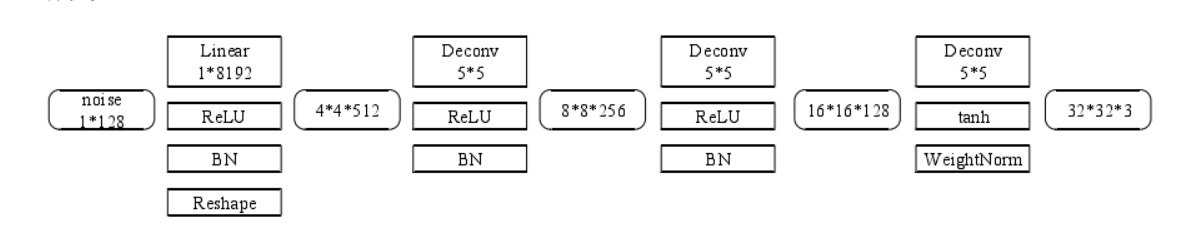
\includegraphics[scale=0.6]{figure/5.2.png}
	\caption{Network architecture}
	\label{f4.2}
\end{figure}
\begin{figure}[H]
    \centering
	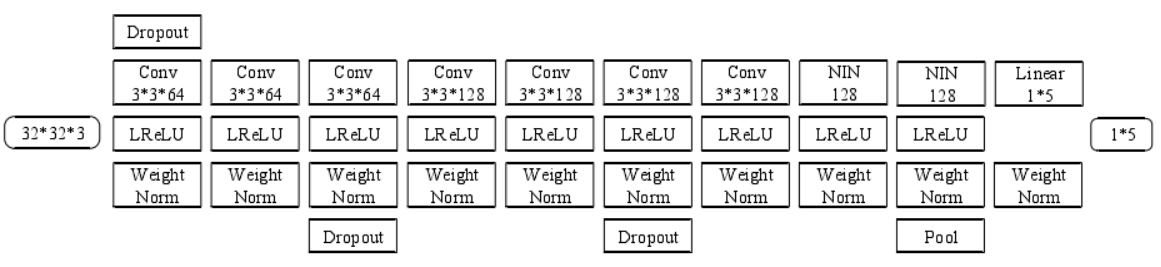
\includegraphics[scale=0.6]{figure/5.3.png}  
	\caption{Classifier Network architecture}
	\label{f4.3}
\end{figure}

As shown in Figure \ref{f4.2}, it is a network structure diagram of the generator in the semi-supervised generation confrontation network. This part generates a pseudo-crop image of a specified size from random noise. Figure \ref{f4.3} shows the network structure of the discriminator in the semi-supervised generative adversarial network. The discriminator is composed of a multi-layer convolutional neural network, which is the semi-supervised generative adversarial network classifier.

\section{Conclusion}
In this article, this paper uses semi-supervised generative adversarial networks to perform semi-supervised learning on crop disease and insect images. We redesigned the network composition of generators and discriminators in generative adversarial networks based on the characteristics of crop images. In the generative confrontation network used, this paper designs a multi-layer generator network and a discriminator deep neural network. The input to generate the adversarial network is the result of the improved network segmentation, combining the artificially selected features with the features calculated by the neural network.

\bibliography{ref}

\end{document}
